\begin{enumerate}[i]
\item The solution of this problem should provided 0/1 labels for each pixel in every frame of the test videos. Label 0 denotes this pixel represents the background in the current frame while label 1 denotes the foreground. We could measure the accuracy of the provided solution by comparing every predicted label against the ground truth of the test videos. A successful solution should provide prediction results should be no worse than the incremental EM solution in \cite{friedman1997image}.
    Moreover, the solution provided by the teams must be online. In order to predict the result, we also need to evaluate the running time to produce labels for a single frame comparing against the total running time. The processing time for each frame for a successful online solution should be roughly the total time divided by the number of frames.
\item In prior work we implemented a form of online expectation
  maximization as inference for a natural probabilistic
  generalization of background subtraction\cite{friedman1997image}.
  (The \emph{model} is a natural 
  generalization; the inference is significantly more
  complicated than taking an average over frames.)  The following two sections
  reproduce that paper's description of background subtraction and our
  generalization of it.
\item There are many existing background substraction datasets. We could use a renderer engine to generate some small synthetic data as well as use a real-world dataset, i.e. the UCSD dataset\footnote{\url{http://www.svcl.ucsd.edu/projects/background_subtraction/ucsdbgsub_dataset.htm}}, for evaluating the performance.
\item The teams should load the video frames from disk and output all the labels for each video frame in a single text file. For example, when the video name is \texttt{A}, then the result for the 1st frame in \texttt{A} should be stored in \texttt{A1.txt}. The evaluation script should load all the labels from the text files and evaluate the predicted accuracy.
\item In the first stage, we will only deliver the small synthetic data. In the second stage, we deliver a small portion of the UCSD dataset to the teams and evaluate the performance using the remaining videos. Another choice for the second stage could be that for each video data in the UCSD dataset, we deliver only the first 25\% to the teams and using the whole video (or the remaining 75\%) for evaluation.
\end{enumerate}


As it turns out, a solution to both difficulties is to first
\emph{classify} and then \emph{selectively update}.  Roughly, only
updating the background image with those pixels presently classified as
belonging to it gives better results.  There are stable and
unstable ways to go about the selective updating; the stable way
hinges on a properly Bayesian treatment of the classification of the
pixels.  In other words, we define a generative
probabilistic model of pixel values given pixel classes; subsequently
the math fully determines, by Bayes Rule, the optimal classification
given observed values.  In practice the implementation must
cut some corners for the sake of feasibility, the details of that are
in the original paper~\cite{friedman1997image}. 




\subsection{Probabilistic Shadow and Background Subtraction}
\label{shadow-and-background-subtraction-section}
\label{pixel-model-section}


Consider a single pixel and the distribution of its values over time.
Some of the time it will be in its ``normal'' background state---for
example, a small area of the road surface. Some of the time it may be
in the shadow of moving vehicles, and some of the time it may be part
of a vehicle. Thus, in the case of traffic surveillance, we can think
of the distribution of values $i_{x,y}$ of a pixel $(x,y)$ as the
weighted sum of three distributions $r_{x,y}$ (road), $s_{x,y}$
(shadow), and $v_{x,y}$ (vehicle):
\[ i_{x,y} = \w_{x,y} \cdot (r_{x,y},\ s_{x,y},\ v_{x,y}) \]
These distributions are subscripted
to emphasize that they differ from pixel to pixel; $r_{x,y}$ is a
probability distribution for the way that {\em this specific pixel}
looks when it is showing unshadowed road at the corresponding physical
location. It is essential to have different models for each pixels,
because, for example, some parts of the image may correspond to white road
markings, others to dark streaks in the centers of lanes, and still
others to lamp-posts (see \figref{fast-traffic-figure}).
The weights are also subscripted, because some pixels
may spend more time in shadow or vehicle than others.

\begin{figure*}[t]
\subfigure[a]{
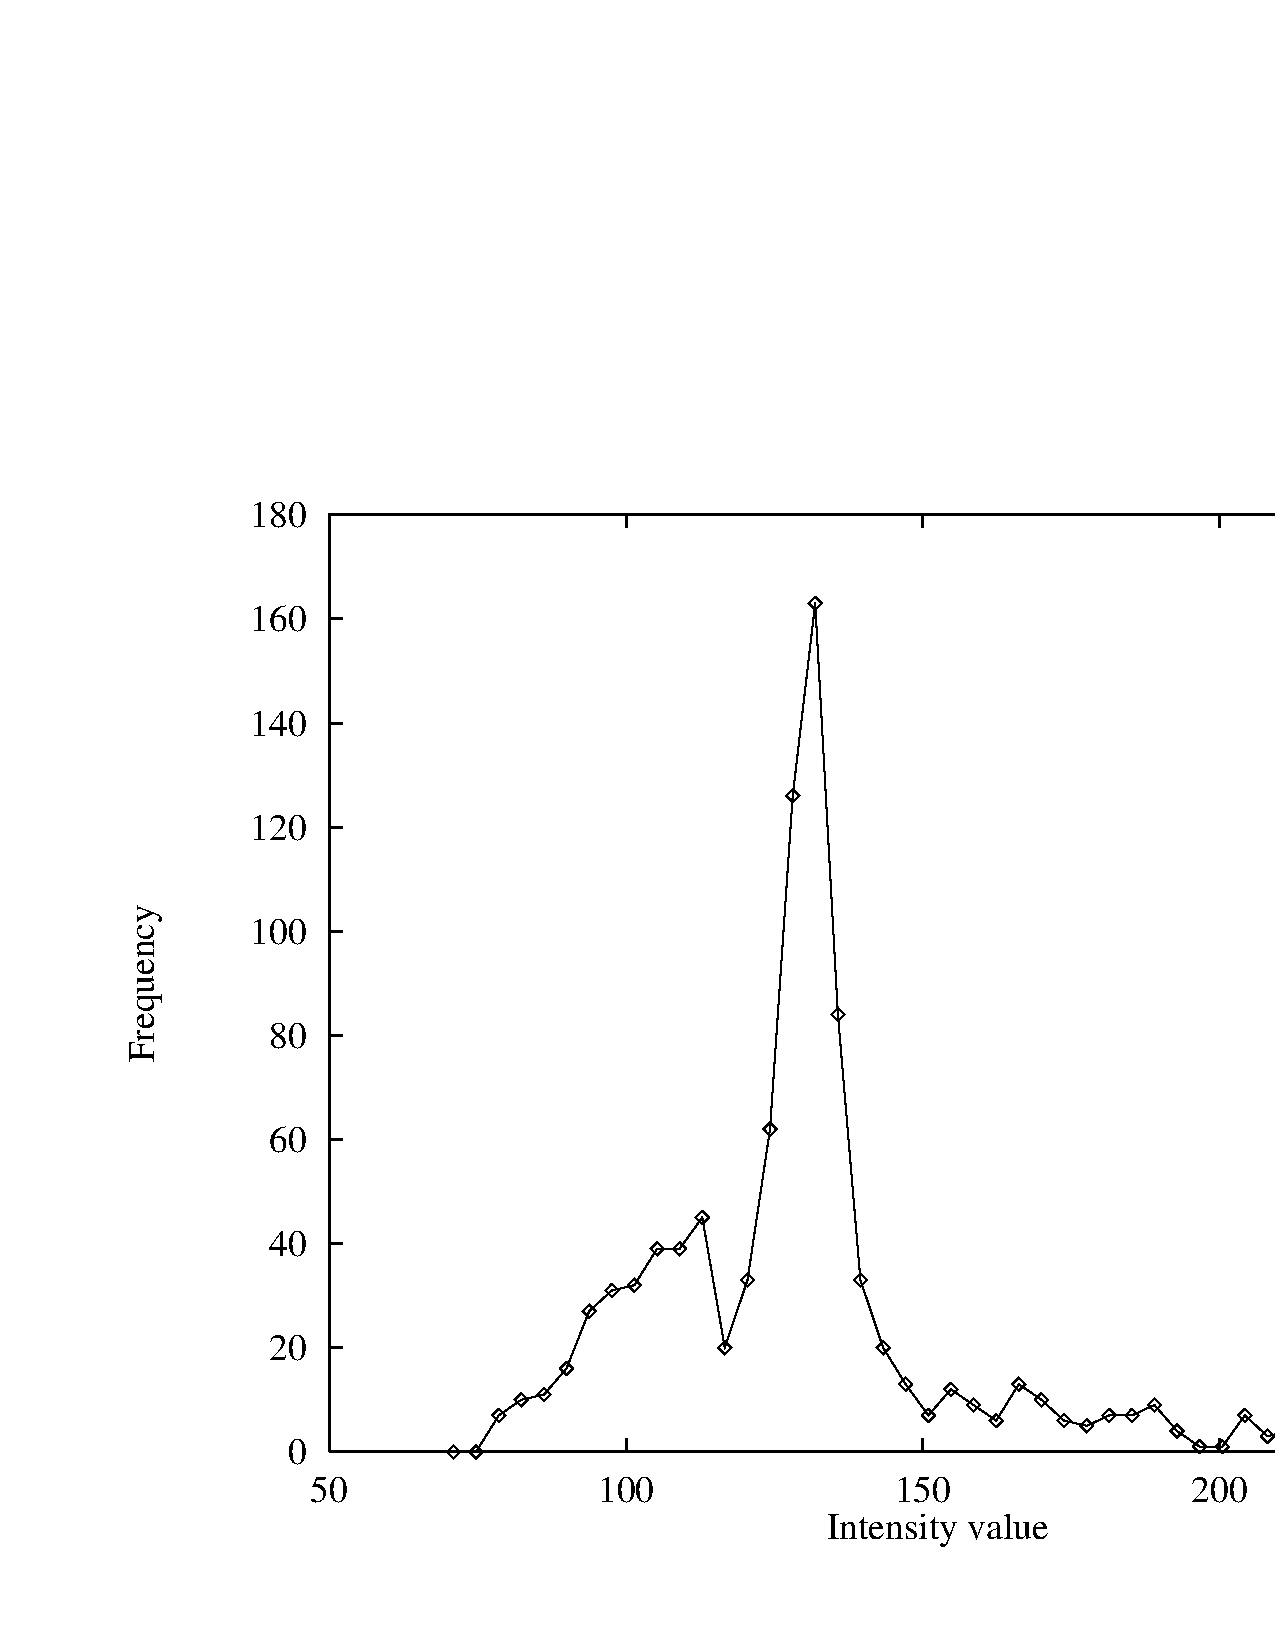
\includegraphics[width=0.23\textwidth]{graphs/intensity-freq.pdf}
}
\subfigure[a]{
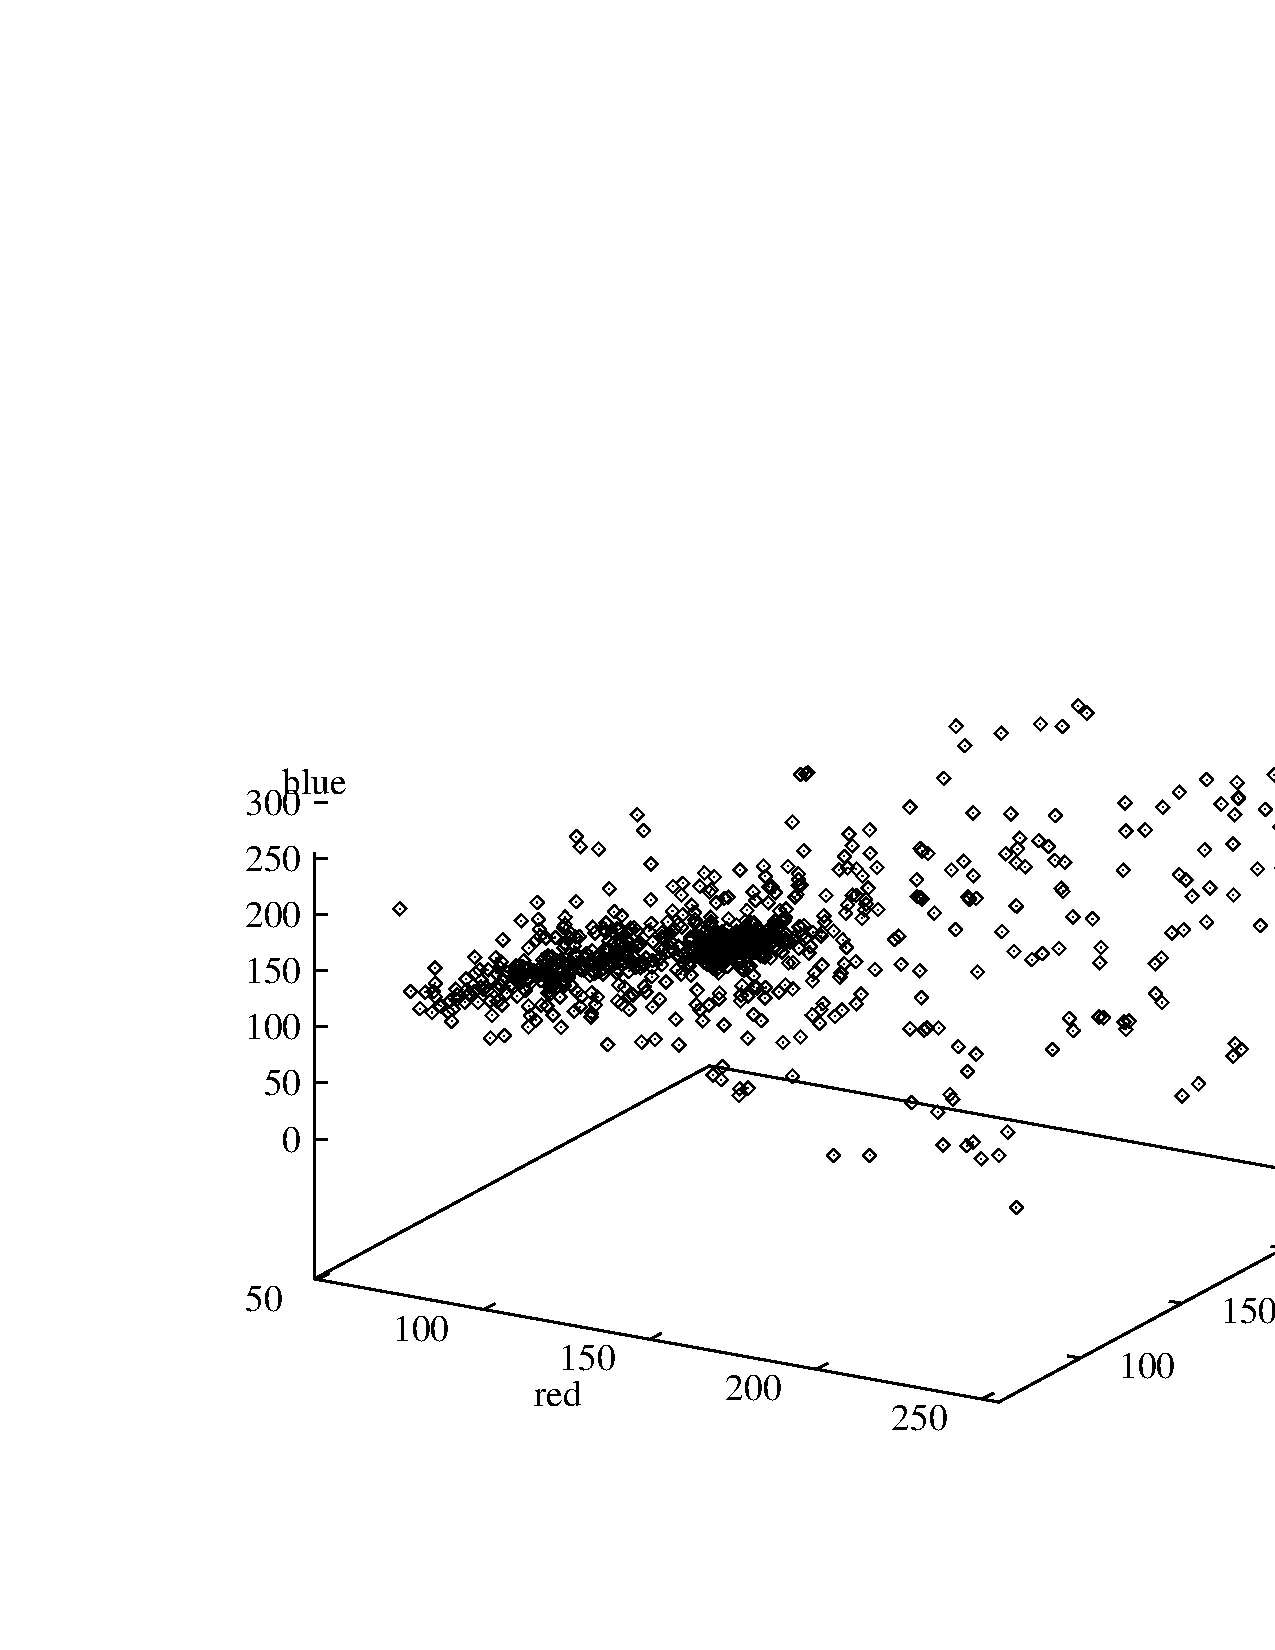
\includegraphics[width=0.23\textwidth]{graphs/rgb-scatter.pdf}
}
\subfigure[a]{
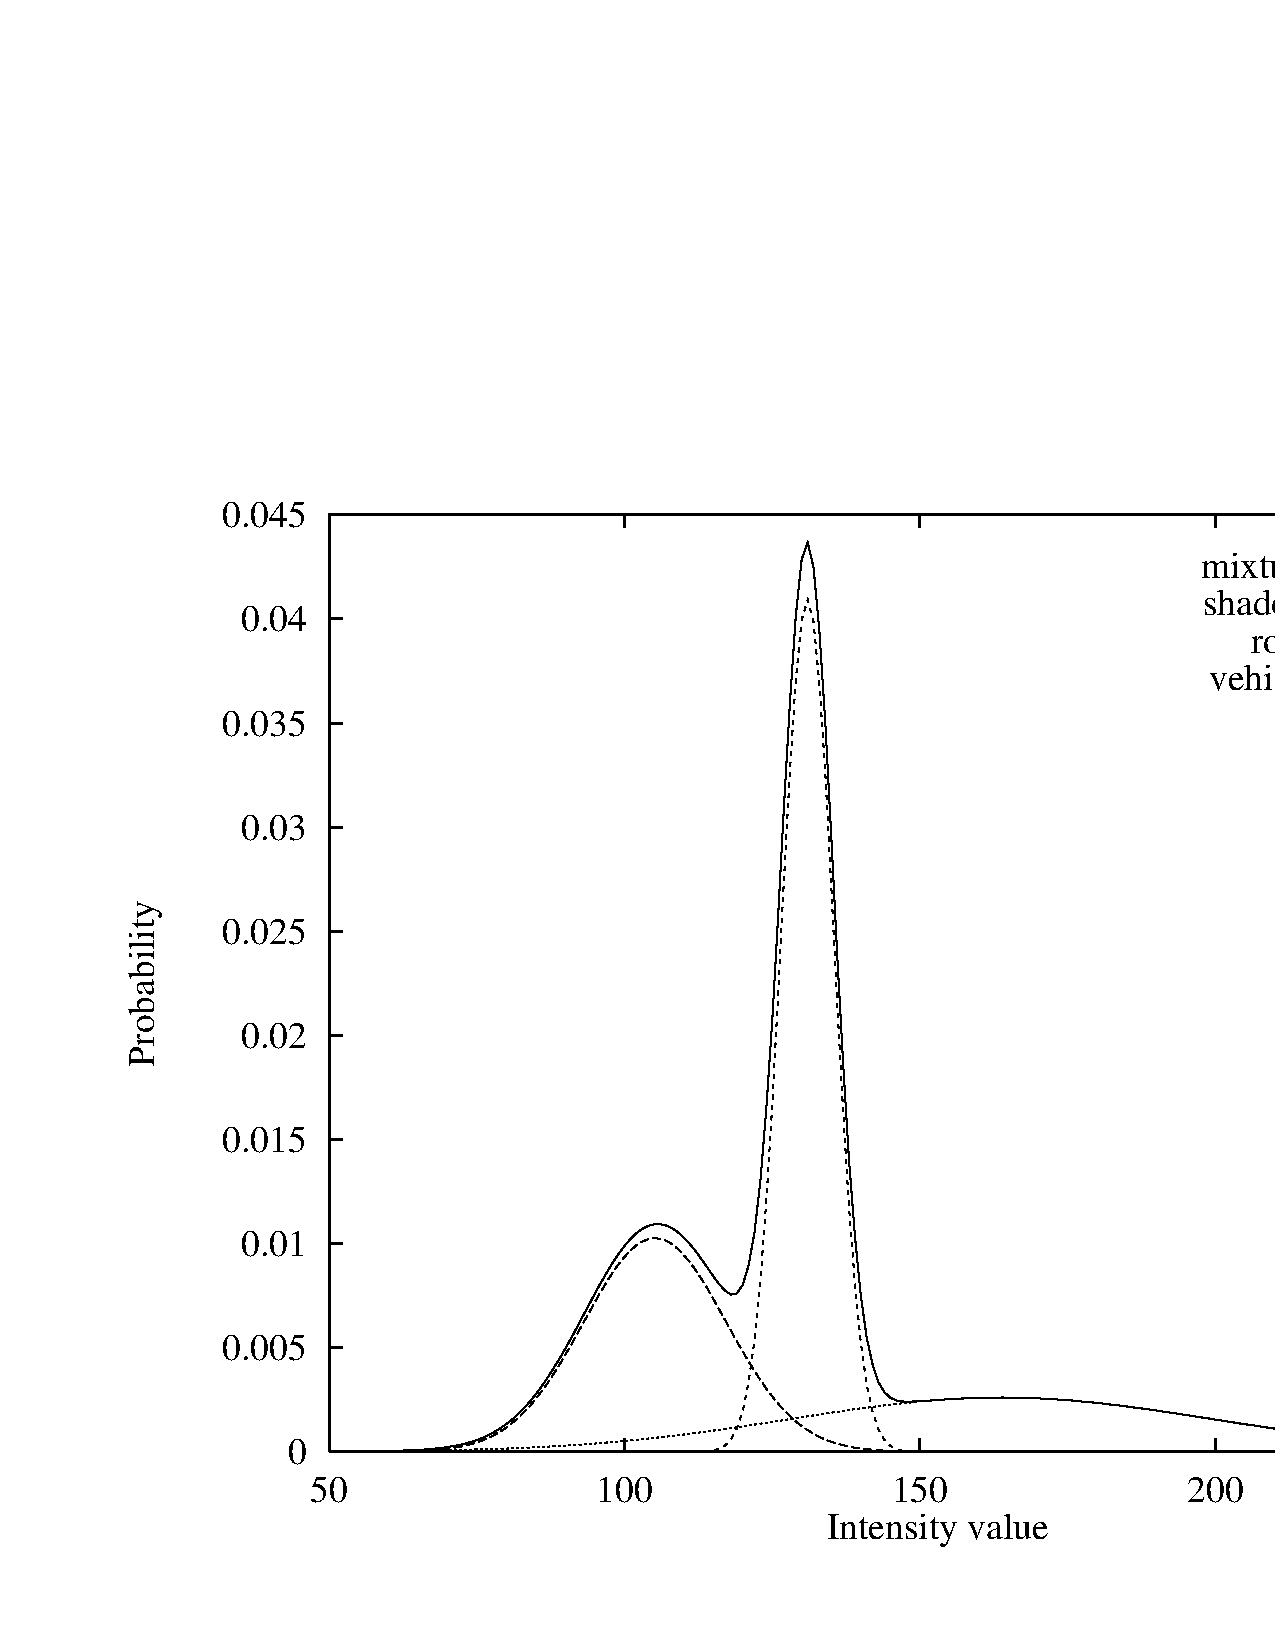
\includegraphics[width=0.23\textwidth]{graphs/intensity-model.pdf}
}
\subfigure[a]{
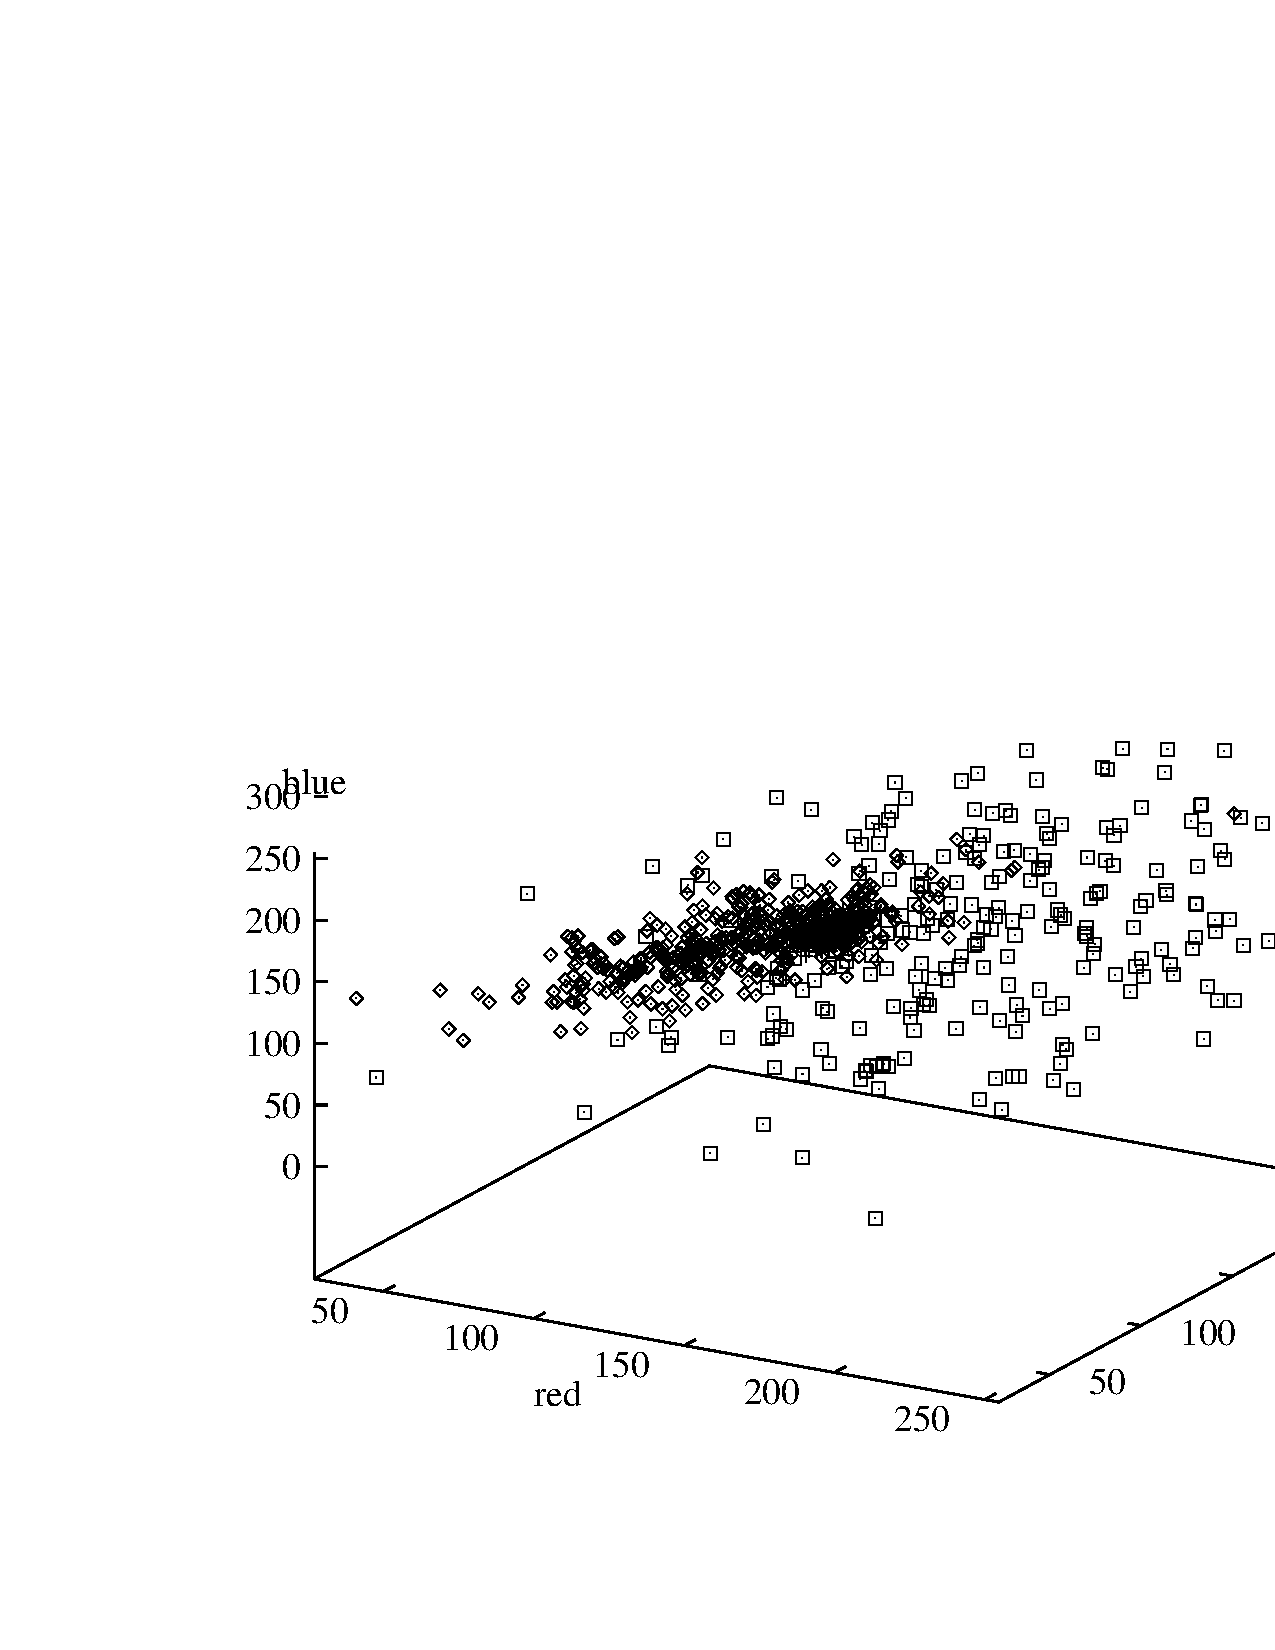
\includegraphics[width=0.23\textwidth]{graphs/rgb-model.pdf}
}
\caption{(a) Empirical distribution of intensity values for pixel (160,170)
over 1000 frames. (b) Scatter plot of RGB values for the same pixel.
(c) Fitted three-component Gaussian mixture model for the data in (a).
(d) Scatter plot of 1000 randomly-generated data points from a fitted
three-component Gaussian mixture model for the data in (b).}
\label{pixel-model-figure}
\end{figure*}

Figures~\ref{pixel-model-figure}(a) and~\ref{pixel-model-figure}(b)
show the empirical distribution of intensity and RGB values,
respectively, for pixel (160,170), which is roughly two-thirds of the
way towards the bottom right corner of the image.  These data display
the behaviour one would expect: the shadow and road pixels form two
fairly well-defined peaks, while the vehicle pixels are widely
scattered.  As a first approximation, we assume that each distribution
can be modelled as a Gaussian.  Using expectation maximization, we can fit three-component mixture models to the
data. \figref{pixel-model-figure}(c) shows the fitted model for
intensity values, and \figref{pixel-model-figure}(d) shows a scatter
plot for the fitted RGB model. The fitted models are reasonably good
(but far from ideal) approximations to the empirical data.

%the techniques described in
%\secref{EM-section},
%%
%% the label problem solution is in {results-section}
%%

The model for pixel $(x,y)$ is parameterized by the parameters $\Theta
= \{
w_l, \mu_l, \Sigma_l : l \in \{ r, s, v \}\}$ so that $\w_{x,y} = (w_r,
w_s, w_v )$, $r_{x,y} \sim N(\mu_r,\Sigma_r)$, and so on.%
\footnote{For clarity, we omit the subscript $x,y$ from the names of
these parameters. However, it should be clear that there is a
different set of parameters for pixel position $x,y$.}
Our models apply in two settings. In the first, we examine intensity
levels, and $\mu$ and $\Sigma$ are scalars. In the second, we examine
RGB values, and $\mu$ is a $3\times 1$ vector and $\Sigma$ is a $3\times 3$
matrix. The derivations are identical in the two cases, so we do not
distinguish between them in the following discussion.

Let $i$ be a pixel value (either an intensity level or a vector of RGB
values). Let $L$ be a random variable denoting the {\em label\/} of
the pixel in this image. Our model defines the probability that $L =
l$ and $I(x,y,t) = i$ to be
\begin{eqnarray*}
\lefteqn{P( L = l, I(x,y,t) = i \mid \Theta ) = {}} \\
 & &  w_l \cdot
(2\pi)^{-\frac{d}{2}}|\Sigma_l|^{-\frac{1}{2}} \exp\{-\frac{1}{2}(i -
\mu_l)^T {\Sigma_l}^{-1} (i - \mu_l)\}
\end{eqnarray*}
where $d$ is the dimension of each pixel value (1 or 3 in our case).
Given these probabilities, we can classify the pixel value. Namely, we
choose the class $l$ with highest posterior  probability $P( L = l \mid I(x,y,t)) $.

